\chapter{Predstavitev sistema}
\label{ch:sistem}

V tem poglavju opišemo delovanje sistema po posameznih modulih: kaj se zgodi, ko uporabnik izvede določeno dejanje v odjemalski aplikaciji, kateri klic proti zaledni aplikaciji to dejanje sproži in kako se odrazi v podatkovni bazi. Zaledna koda je razdeljena na module po domenah: avtentikacija, zaposleni, izmene, razporejanje, odsotnosti, dogodki, obiski in administracija. Vsak modul izpostavi svoj nabor poti REST znotraj skupne aplikacije, opisane v razdelku~\ref{sec:arhitektura}.

Slika~\ref{fig:manager-prijava} prikazuje prijavno stran spletne aplikacije za vodje in kadrovsko službo. Enak vzorec obrazca (elektronski naslov, geslo) uporabljajo tudi ostale spletne aplikacije, opisane v nadaljevanju poglavja.

\begin{figure}[htbp]
\centering
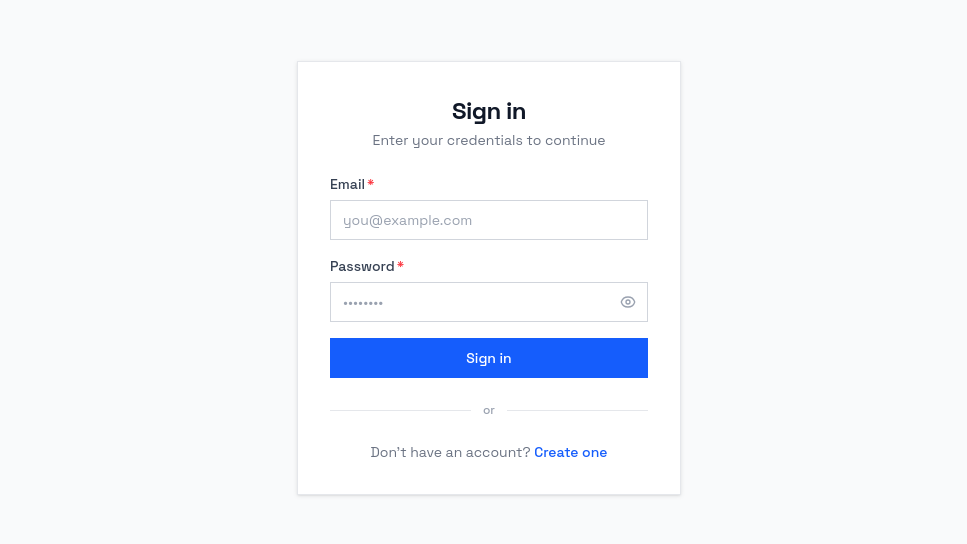
\includegraphics[width=\textwidth]{slike/manager-prijava.png}
\caption{Prijavna stran spletne aplikacije za vodje in kadrovsko službo.}
\label{fig:manager-prijava}
\end{figure}
\FloatBarrier

\section{Avtentikacija in nadzor dostopa}
\label{sec:sistem-avtentikacija}

Nova organizacija pridobi zaposlene prek povabil: kadrovska služba na naslov zaposlenega pošlje povabilo, ki ga zaledje shrani v tabelo \texttt{invitations} skupaj z zgoščeno vrednostjo enkratnega žetona. Zaposleni ob sprejemu povabila izbere geslo, zaledje pa ob prijavi preveri elektronski naslov z enkratno kodo (angl. One-Time Password, OTP), ki jo pošlje po elektronski pošti prek čakalne vrste, opisane v razdelku~\ref{sec:arhitektura}. Zaledje po petih zaporednih napačnih poskusih vnosa kode nadaljnje poskuse zavrne in zahteva ponoven začetek registracije, potekle ali že uporabljene kode pa zavrne takoj.

Ob uspešni prijavi zaledje izda dva žetona JWT: kratkoživ dostopni žeton, ki ga odjemalec hrani v pomnilniku in ga pošilja v glavi \texttt{Authorization}, ter dolgoživ osvežitveni žeton, ki ga zaledje shrani kot sejo (\texttt{sessions}) in odjemalcu vrne v piškotku, vezanem na napravo. Taka delitev omeji izpostavljenost dostopnega žetona, hkrati pa uporabniku ni treba gesla vnašati znova ob vsakem poteku dostopnega žetona. Ker si spletna aplikacija za vodje in administratorska aplikacija delita isto zaledno domeno, zaledje piškotka za navadne uporabnike in administratorja loči po imenu, dostopni žeton v glavi \texttt{Authorization} pa ima vedno prednost pred piškotkom, da preprečimo, da bi zastarel piškotek ene aplikacije preglasil žeton druge.

Vsak klic na zaščiteno pot gre skozi dve zaporedni varovali. Prvo (\texttt{JwtAuthGuard}) preveri veljavnost dostopnega žetona in iz njega prebere identiteto ter vlogo uporabnika. Poti, označene kot javne, preverjanje preskočijo. Drugo (\texttt{RolesGuard}) preveri, ali vloga uporabnika ustreza vlogam, ki jih zahteva klicana pot, sicer zahtevo zavrne s stanjem 403. Tabela~\ref{tab:vloge} povzame, katere vloge imajo dostop do posameznih sklopov funkcionalnosti.

\begin{table}[htbp]
\centering
\caption{Poenostavljen pregled dostopa do posameznih sklopov po vlogah.}
\label{tab:vloge}
\resizebox{\textwidth}{!}{%
\begin{tabular}{lccccc}
\toprule
Sklop & Admin & HR & Vodja & Zaposleni & Superadmin \\
\midrule
Lastni dogodki, izmene, odsotnosti & \checkmark & \checkmark & \checkmark & \checkmark & -- \\
Urejanje izmen tima & \checkmark & \checkmark & \checkmark & -- & -- \\
Nastavitve razporejanja & \checkmark & \checkmark & -- & -- & -- \\
Upravljanje zaposlenih in povabil & \checkmark & \checkmark & \checkmark & -- & -- \\
Potrjevanje odsotnosti in popravkov & \checkmark & \checkmark & \checkmark & -- & -- \\
Organizacije čez celotno platformo & -- & -- & -- & -- & \checkmark \\
\bottomrule
\end{tabular}%
}
\end{table}
\FloatBarrier

\section{Upravljanje zaposlenih}
\label{sec:sistem-zaposleni}

Kadrovska služba v spletni aplikaciji ustvari povabilo z elektronskim naslovom, imenom, priimkom in vlogo novega sodelavca. Zaledje ustvari zapis v tabeli \texttt{invitations} in po čakalni vrsti odloži pošiljanje elektronske pošte s povezavo do sprejema povabila. Ko zaposleni povabilo sprejme in izbere geslo, zaledje ustvari nov zapis v tabeli \texttt{users} z ustrezno vlogo in organizacijo ter pripadajoč \texttt{employee\_profiles} z osnovnimi kadrovskimi podatki, povabilo pa označi kot sprejeto. Kadrovska služba lahko kadar koli pregleduje seznam zaposlenih, ureja podatke posameznega profila (delovno mesto, oddelek, najvišje tedensko število ur) ali prekliče še nesprejeto povabilo.

\section{Evidenca delovnega časa}
\label{sec:sistem-cas}

Zaposleni v mobilni aplikaciji ob prihodu, odhodu, začetku ali koncu odmora ter podobnih dogodkih sproži enostaven klic, ki v tabelo \texttt{work\_events} doda vrstico s tipom dogodka in časovnim žigom. Ker se dogodki beležijo sproti in je napačen pritisk pogost, zaposleni namesto neposrednega urejanja že zabeleženega dogodka odda zahtevek za popravek: ta se shrani v tabelo \texttt{event\_change\_requests} skupaj z zahtevanim tipom dogodka, časom in razlogom, obstoječi dogodek pa ostane nespremenjen do odobritve. Vodja v spletni aplikaciji pregleduje čakajoče zahtevke svojega tima. Ob odobritvi zaledje glede na vrsto zahtevka (dodaj, uredi, izbriši) ustrezno spremeni izvorni zapis v \texttt{work\_events} in zahtevek označi kot odobren, ob zavrnitvi pa zgolj zabeleži razlog in izvorni dogodek pusti nespremenjen.

\section{Razporejanje izmen}
\label{sec:sistem-razporejanje}

Vodja urnik lahko sestavlja ročno, izmeno po izmeno, ali s ponavljajočimi se vzorci in predlogami zasedenosti, opisanimi v razdelku~\ref{sec:podatkovni-model}. Izmena brez dodeljenega zaposlenega je označena kot odprta, kateri koli ustrezen zaposleni jo lahko v mobilni ali spletni aplikaciji prevzame, zaledje pa ob tem preveri, da se izmena ne prekriva z že dodeljenimi izmenami tega zaposlenega. Slika~\ref{fig:manager-urnik} prikazuje tedenski pregled urnika v spletni aplikaciji za vodje.

\begin{figure}[htbp]
\centering
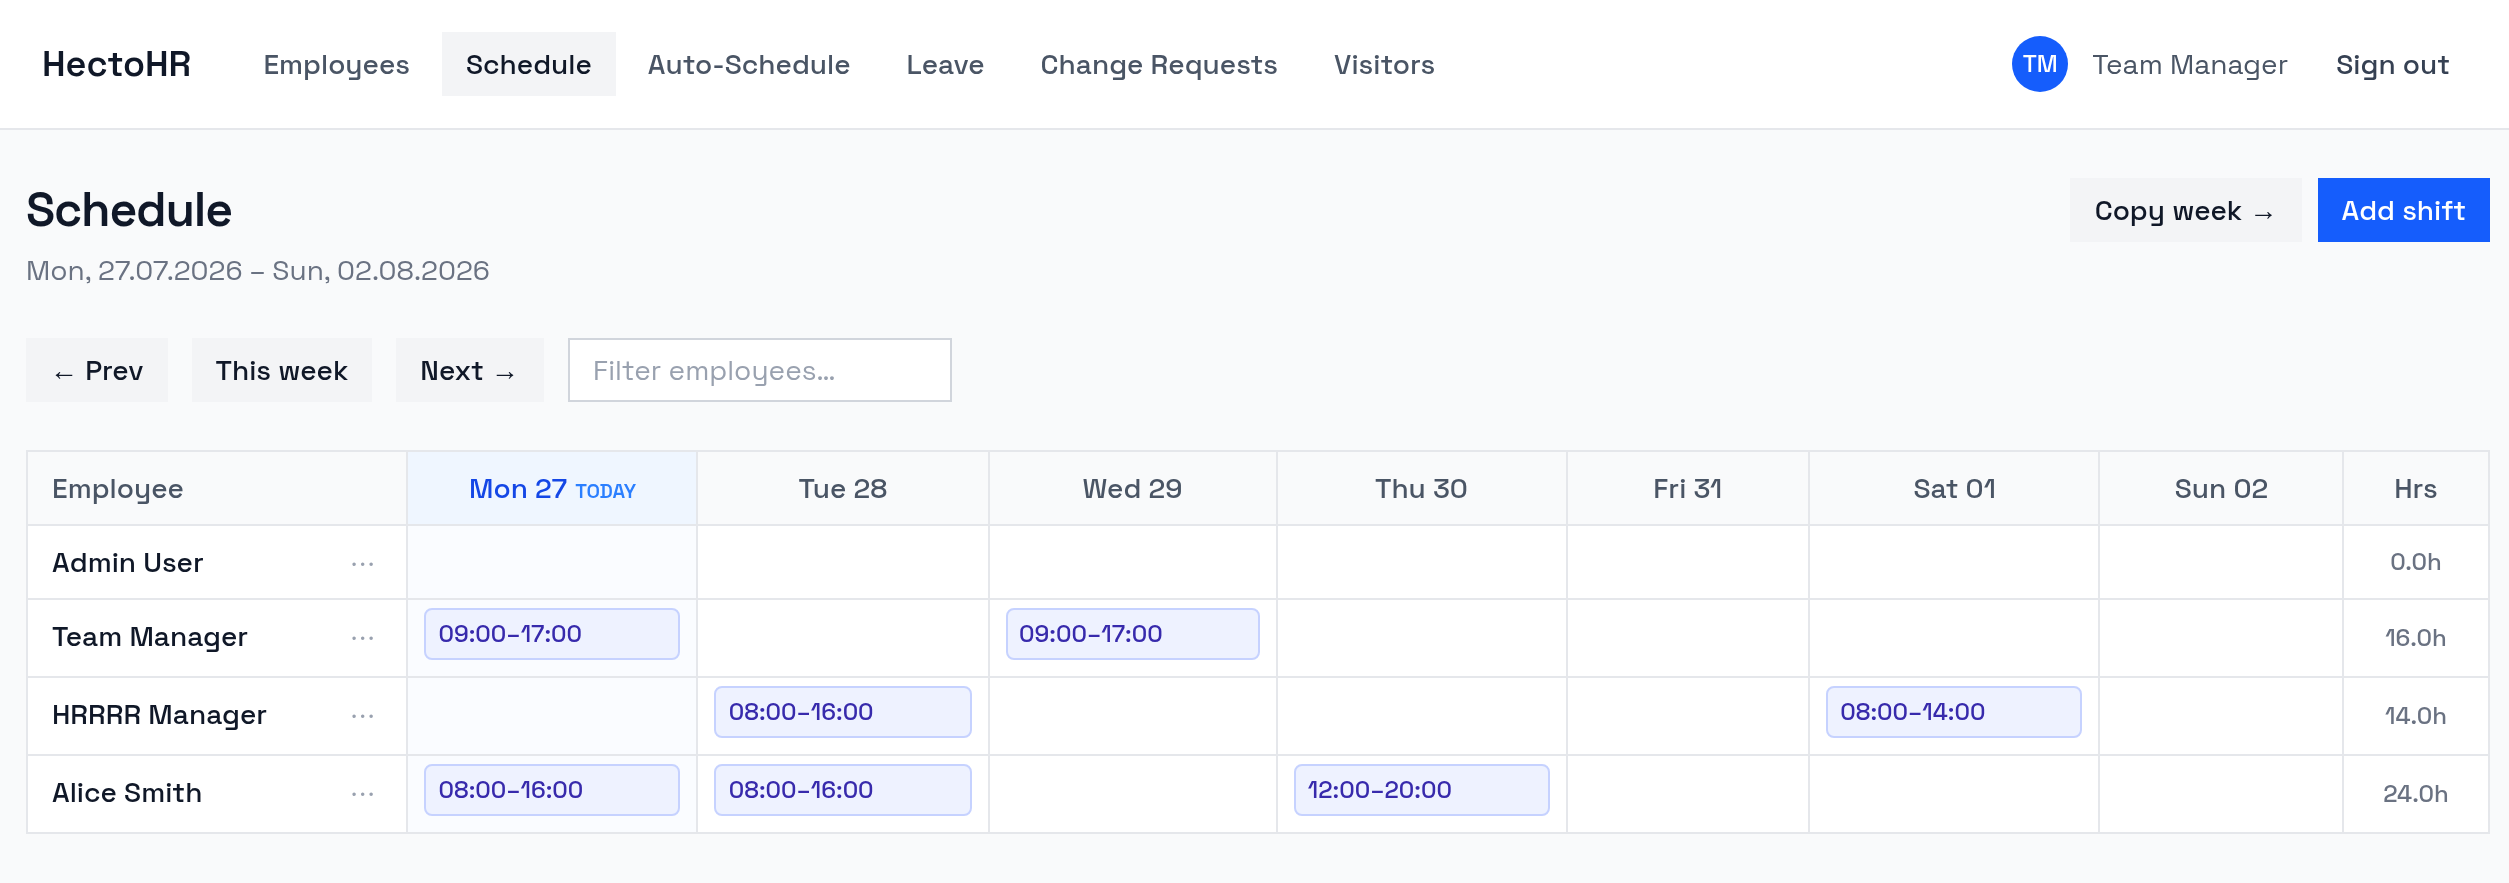
\includegraphics[width=\textwidth]{slike/manager-urnik.png}
\caption{Tedenski pregled urnika v spletni aplikaciji za vodje.}
\label{fig:manager-urnik}
\end{figure}
\FloatBarrier

Za samodejno sestavljanje urnika vodja izbere časovno obdobje, za katero želi predlog. Zaledje najprej iz predlog zasedenosti za to obdobje ustvari manjkajoče izmene, nato pa ustvari osnutek urnika (\texttt{schedule\_drafts}) in nad njim požene reševalnik. Reševalnik izmene obravnava kronološko in za vsako izmeno med kandidati izbere najprimernejšega zaposlenega, kot prikazuje algoritem~\ref{alg:solver}.

\begin{algorithm}[htbp]
\caption{Poenostavljen potek požrešnega reševalnika razporejanja}
\label{alg:solver}
\begin{algorithmic}[1]
\Function{RazporediOsnutek}{izmene, zaposleni, nastavitve}
    \State razvrsti \textit{izmene} kronološko po datumu in času začetka
    \State stanje $\gets$ prazna preslikava (zasedeni termini in tedenske ure na zaposlenega)
    \For{vsako izmeno $s$ v \textit{izmenah}}
        \State ocene $\gets$ []
        \For{vsakega zaposlenega $z$ v \textit{zaposlenih}}
            \State izračunaj primernost $z$ za $s$: odsotnosti, razpoložljivost, prekrivanje, tedenska omejitev ur, minimalni počitek
            \State ocene.dodaj(($z$, primeren?, preferenca, tedenske ure))
        \EndFor
        \State primerni $\gets$ filtriraj ocene po primeren?
        \If{primerni ni prazen}
            \State najboljši $\gets$ tisti z najvišjo preferenco (izbrana strategija razveže neodločeno po tedenskih urah)
            \State dodeli $s$ najboljšemu, posodobi njegovo stanje
        \Else
            \State označi $s$ kot nezasedeno, zabeleži razlog (npr.\ ni razpoložljivega zaposlenega)
        \EndIf
    \EndFor
    \State \Return predlagane dodelitve
\EndFunction
\end{algorithmic}
\end{algorithm}
\FloatBarrier

Organizacija lahko izbere eno izmed treh strategij razvrščanja, ki določajo, kateremu kriteriju reševalnik pri izbiri med primernimi zaposlenimi da prednost:

\begin{itemize}
    \item \texttt{preference\_first} -- reševalnik najprej izbere zaposlenega z najvišjo preferenco za dani termin, med enako preferenčnimi zaposlenimi pa tistega z manj že dodeljenimi urami v tednu.
    \item \texttt{fairness\_first} -- obrne vrstni red kriterijev: prednost dobi zaposleni z manj že dodeljenimi urami v tednu, preferenca pa odloči šele, če imata dva zaposlena enako število ur.
    \item \texttt{preference\_only} -- razvršča enako kot \texttt{preference\_first}, a med primerne za dani termin uvrsti le tiste zaposlene, ki so ga izrecno označili kot preferiranega, s čimer se preferenca upošteva strogo, ne le kot kriterij razvrščanja.
\end{itemize}

Ker gre za požrešno hevristiko in ne za eksaktni reševalnik, kot smo utemeljili v razdelku~\ref{sec:razporejanje-osebja}, dobljeni osnutek ni nujno optimalen: vodja ga v spletni aplikaciji lahko pregleda, posamezne dodelitve ročno spremeni in šele nato objavi. Slika~\ref{fig:manager-samodejno-razporejanje} prikazuje osnutek urnika za en teden, kjer je reševalnik vseh deset izmen uspešno dodelil štirim zaposlenim, vsako izmeno enemu izmed njih. Med objavo zaledje vsem zaposlenim z dodeljeno izmeno po čakalni vrsti pošlje potisno obvestilo, če pa to ni mogoče, obvestilo pošlje po elektronski pošti.

\begin{figure}[htbp]
\centering
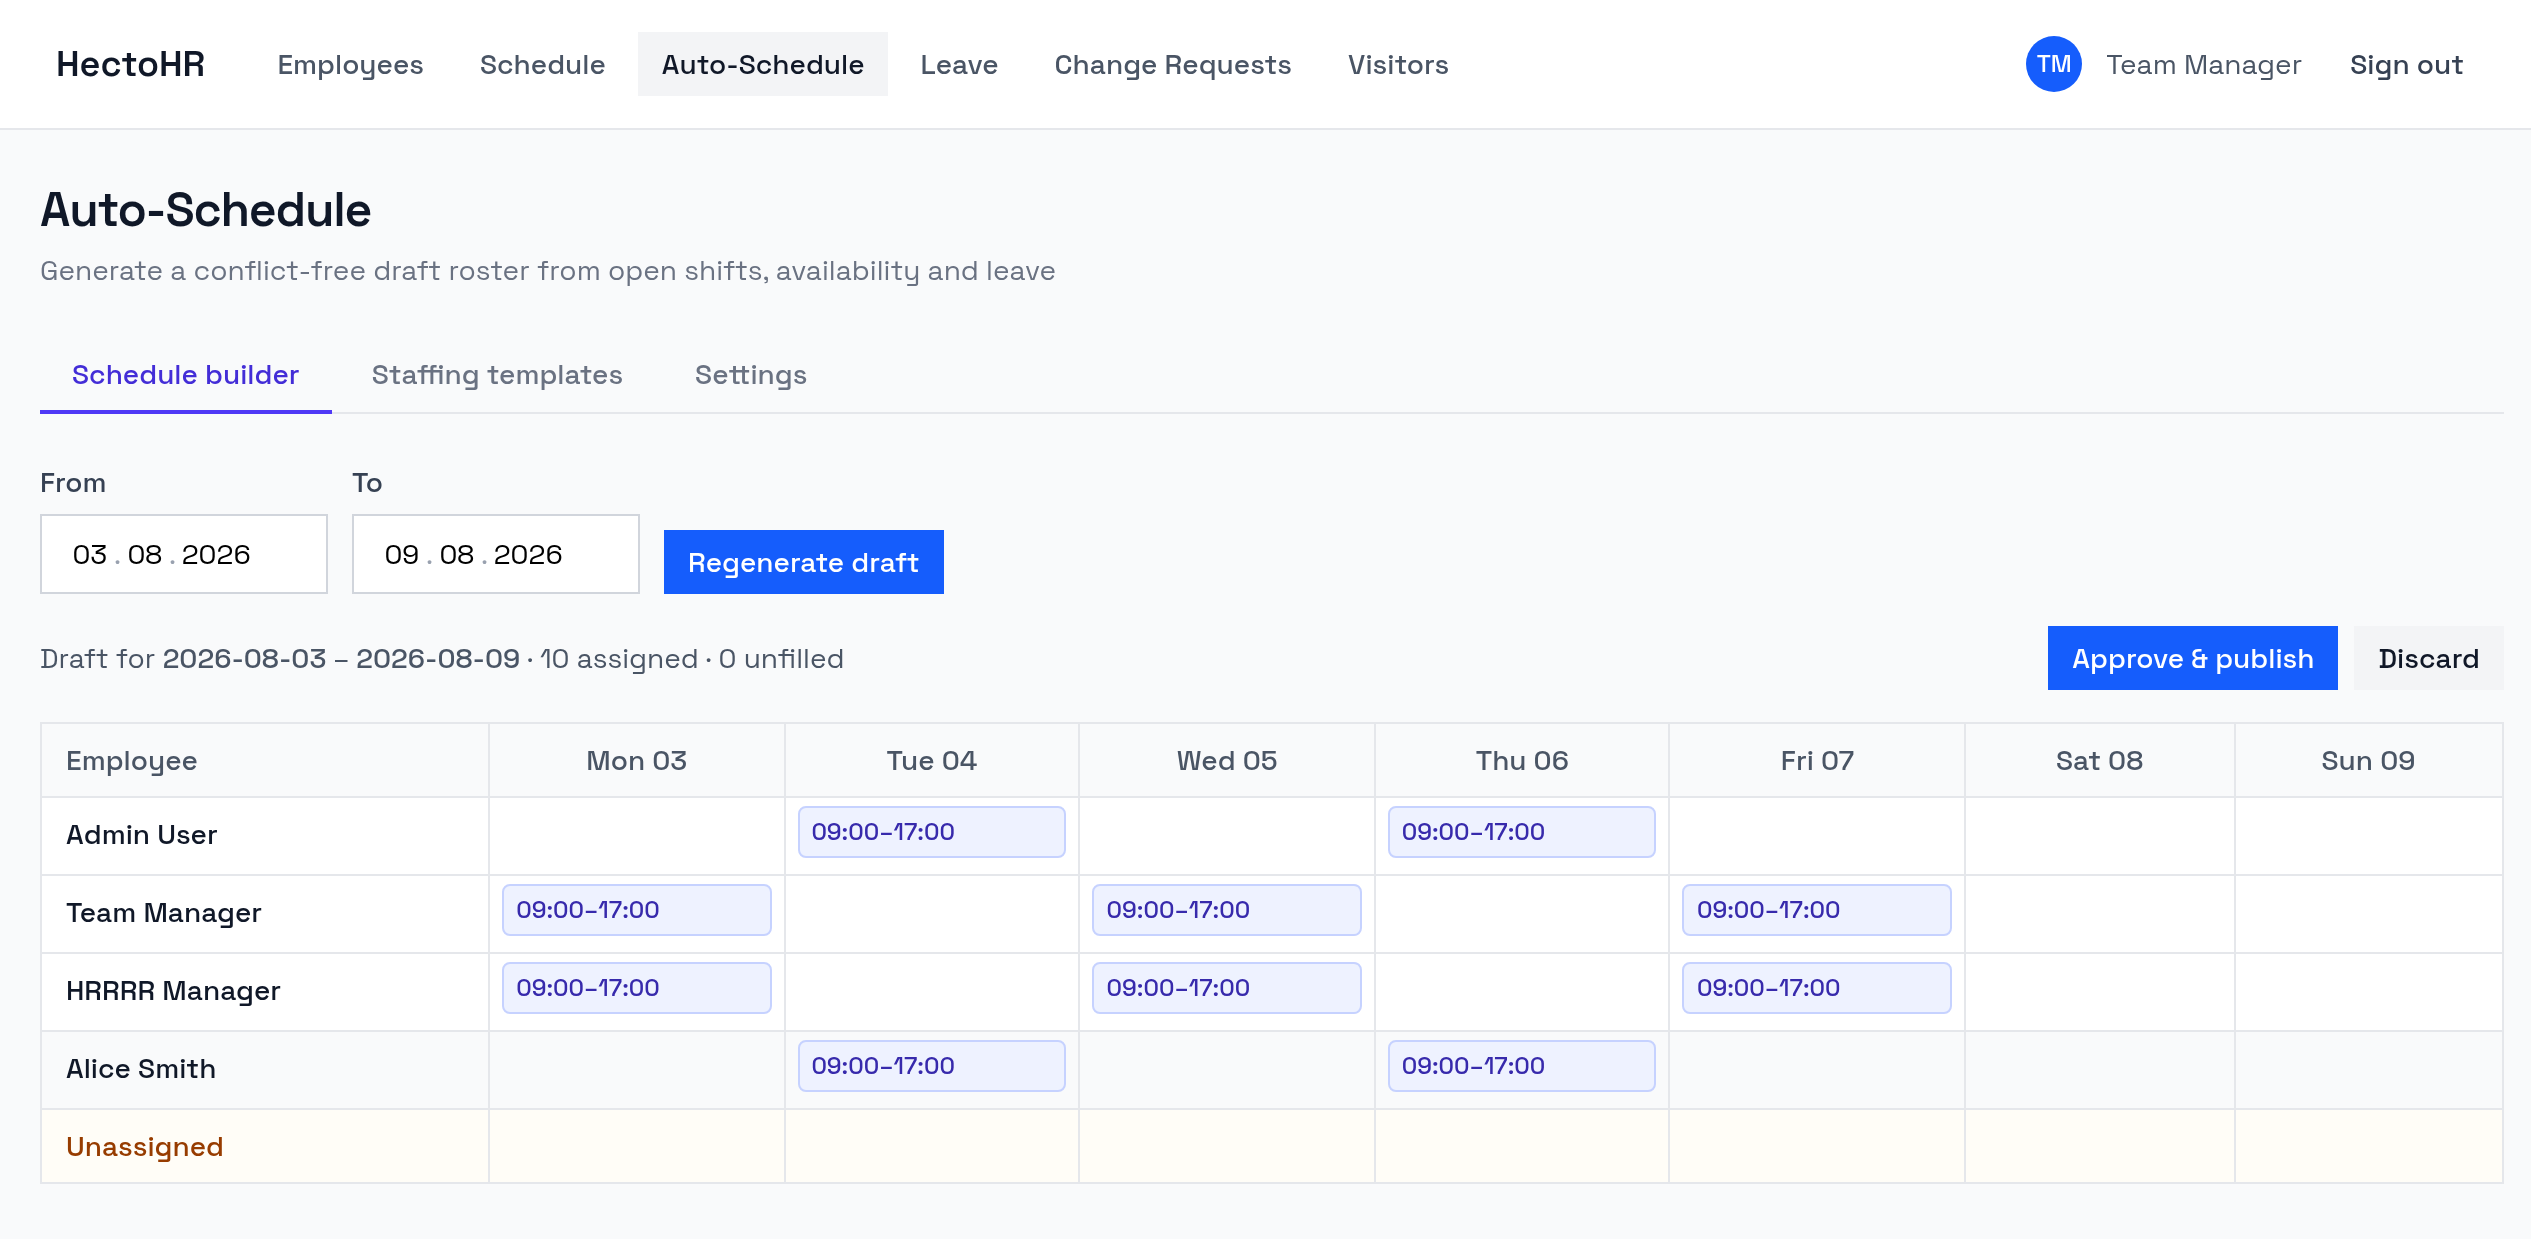
\includegraphics[width=\textwidth]{slike/manager-samodejno-razporejanje.png}
\caption{Osnutek urnika, ki ga je predlagal reševalnik za samodejno razporejanje.}
\label{fig:manager-samodejno-razporejanje}
\end{figure}
\FloatBarrier

\section{Upravljanje odsotnosti}
\label{sec:sistem-odsotnosti}

Kadrovska služba za organizacijo nastavi tipe odsotnosti (na primer letni dopust, bolniška odsotnost) z lastnostmi, ali je tip plačan in koliko dni na leto pripada posameznemu zaposlenemu privzeto. Zaledje nato za vsakega zaposlenega in leto ustvari ustrezen zapis stanja odsotnosti (\texttt{leave\_balances}). Zaposleni v mobilni aplikaciji odda zahtevek za odsotnost z izbranim tipom in obdobjem, zaledje pa samodejno izračuna število delovnih dni in stanje označi kot čakajoče. Vodja ali kadrovska služba zahtevek odobri ali zavrne. Ob odobritvi zaledje čakajoče dni prenese med izrabljene, ob zavrnitvi pa jih vrne nazaj v razpoložljivo stanje. Kadrovska služba lahko dneve v stanju odsotnosti tudi ročno popravi, na primer ob prenosu neizrabljenih dni iz preteklega leta. Slika~\ref{fig:manager-odsotnosti} prikazuje pregled čakajočih zahtevkov za odsotnost v spletni aplikaciji za vodje, skupaj z gumboma za odobritev in zavrnitev.

\begin{figure}[htbp]
\centering
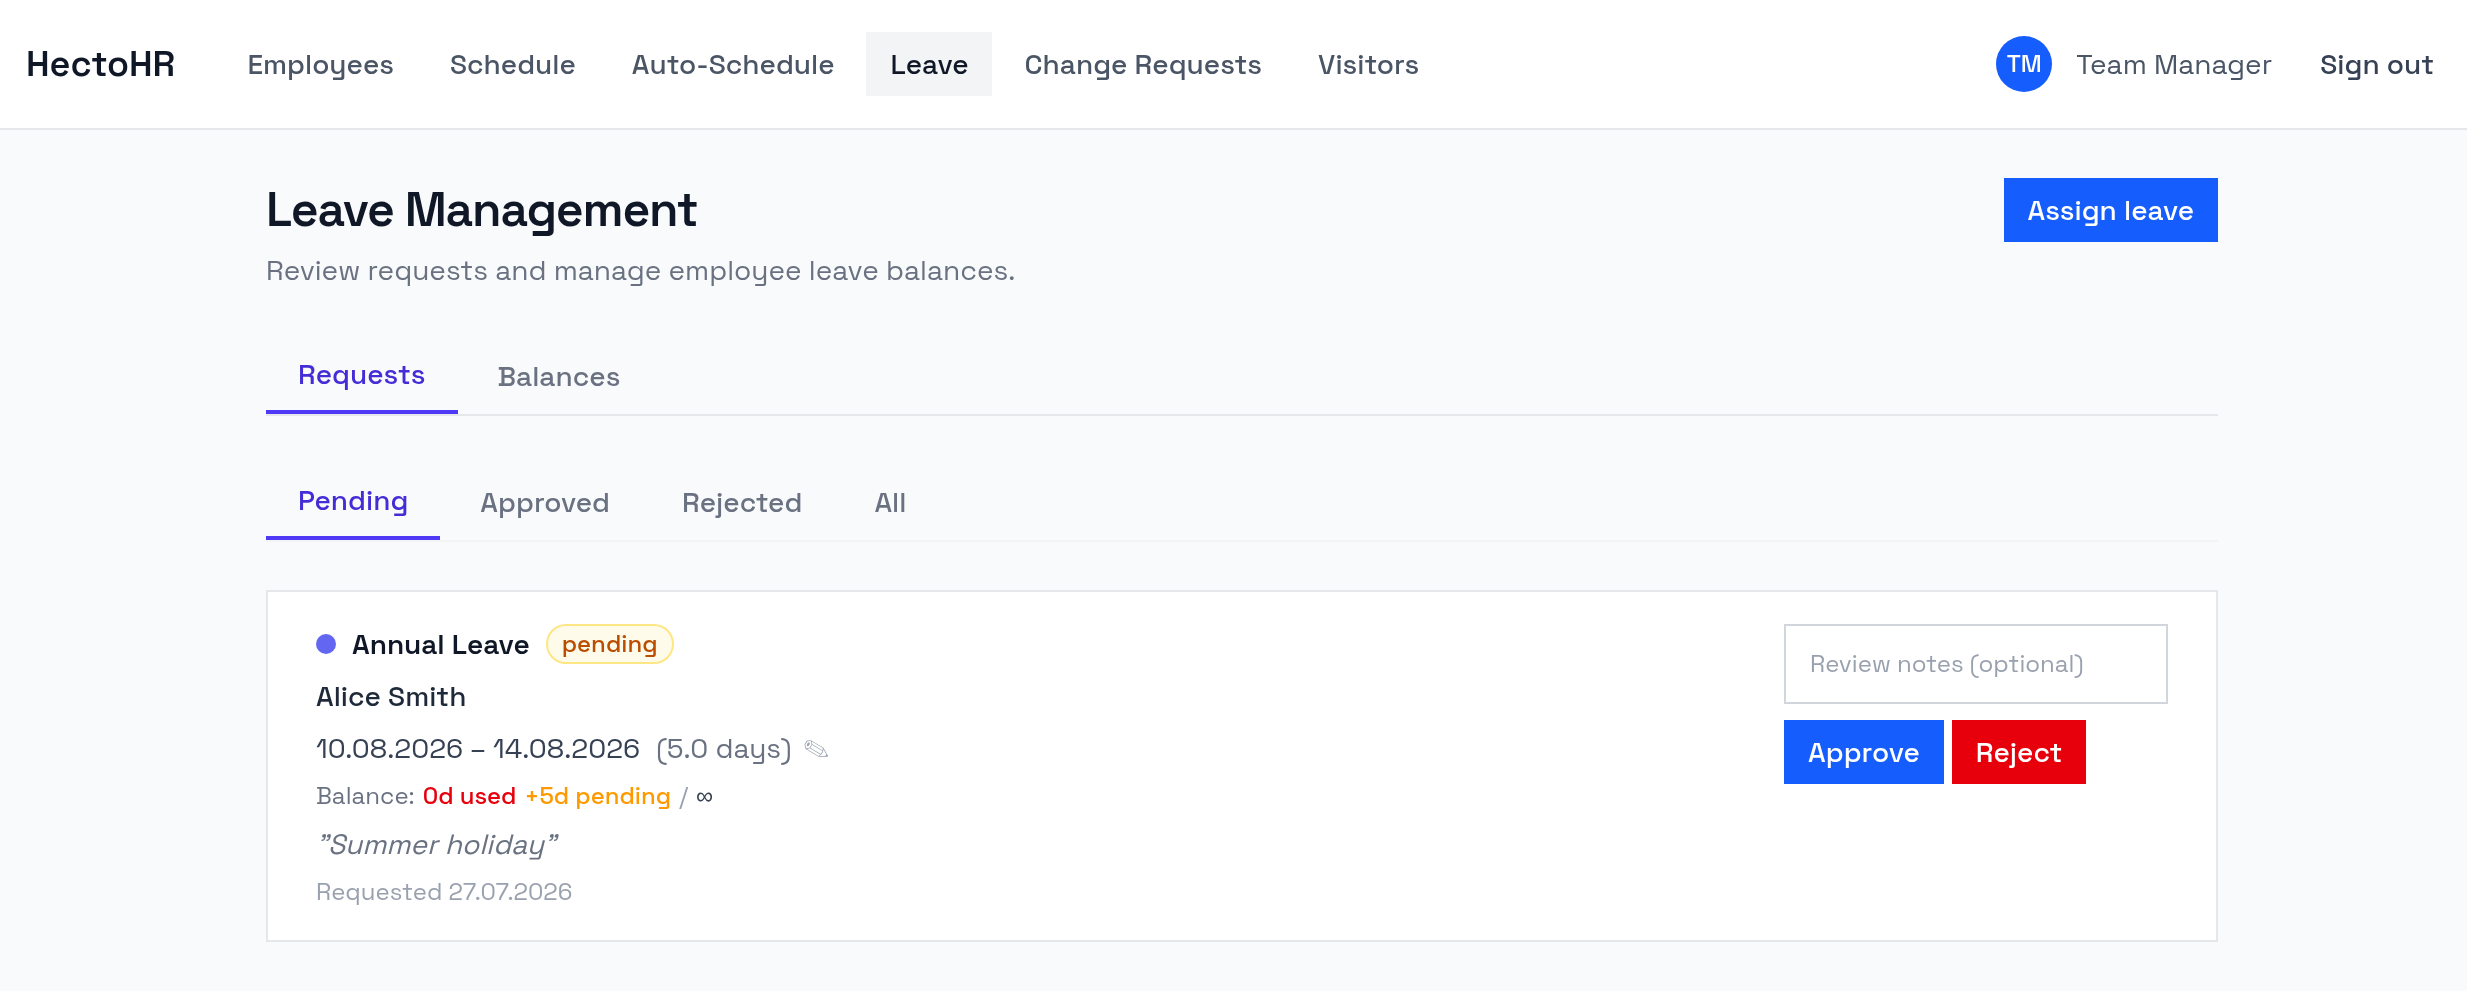
\includegraphics[width=\textwidth]{slike/manager-dopusti.png}
\caption{Pregled čakajočih zahtevkov za odsotnost.}
\label{fig:manager-odsotnosti}
\end{figure}
\FloatBarrier

\section{Evidenca obiskov}
\label{sec:sistem-obiski}

Poleg osrednjih kadrovskih procesov sistem vključuje še dodaten, samostojen modul za evidenco obiskov na recepciji organizacije, ki smo ga omenili že v uvodu (razdelek~\ref{sec:cilji}). Modul teče kot mobilna aplikacija na poljubni napravi na recepciji, najpogosteje tablici, ki jo je treba pred uporabo z zaledjem enkratno seznaniti (parjenje), s čimer vzpostavi lastno zaupanje do zaledja, neodvisno od uporabniške prijave.

Administrator organizacije v spletni aplikaciji ustvari paritveno kodo z omejeno veljavnostjo in imenom naprave (na primer ``Recepcija''), to kodo pa nato enkratno vnese v kiosk aplikacijo na tablici. Zaledje ob uspešnem parjenju kodo porabi in tablici izda dolgoživ žeton naprave, ki ga kiosk aplikacija odslej pošilja namesto uporabniškega žetona JWT. Poti \texttt{/kiosk/*} so zato v celoti izvzete iz varoval, opisanih v razdelku~\ref{sec:sistem-avtentikacija}, in namesto tega preverjajo izključno veljavnost žetona naprave. S tem se izognemo temu, da bi moral vsak obiskovalec za enkraten obisk imeti svoj uporabniški račun.

Obiskovalec na tablici vnese ime in namen obiska ter se podpiše na zaslon, kiosk aplikacija podpis kot sliko naloži neposredno v objektno shrambo, opisano v razdelku~\ref{sec:arhitektura}, zaledje pa ustvari zapis obiska (tabela \texttt{visits}) s časom prihoda in sklicem na naloženo sliko. Recepcija obiskovalca ob odhodu na tablici označi kot odjavljenega, če pa to pozabi, zaledje obisk samodejno zapre ob koncu dne. Zaposleni z ustrezno vlogo lahko v spletni aplikaciji kadar koli preverijo, kdo je trenutno v prostorih organizacije, in pregledajo pretekle obiske.

\section{Administracija platforme}
\label{sec:sistem-admin}

Administrator platforme (vloga \texttt{superadmin}) do sistema dostopa prek ločenega prijavnega mesta, ki sprejme le uporabnike s to vlogo. Ta uporabnik ne pripada nobeni organizaciji in ni ustvarjen prek običajnega vabila, temveč izključno prek namenskega ukaza ob namestitvi sistema. Administratorska aplikacija administratorju omogoča iskanje in pregled organizacij, kar prikazuje slika~\ref{fig:admin-organizacije}, ter uporabnikov čez celotno platformo, onemogočanje ali izbris organizacije, ki posledično prijavo uporabnikom te organizacije zavrne, ter prisilno odjavo ali ponastavitev gesla posameznega uporabnika. Vsako spremembo, ki jo administrator izvede, zaledje zabeleži v tabelo \texttt{admin\_audit\_logs} skupaj s stanjem zapisa pred spremembo in po njej, kar omogoča poznejšo sledljivost posegov, zahtevano v razdelku~\ref{sec:zahteve}.

\begin{figure}[htbp]
\centering
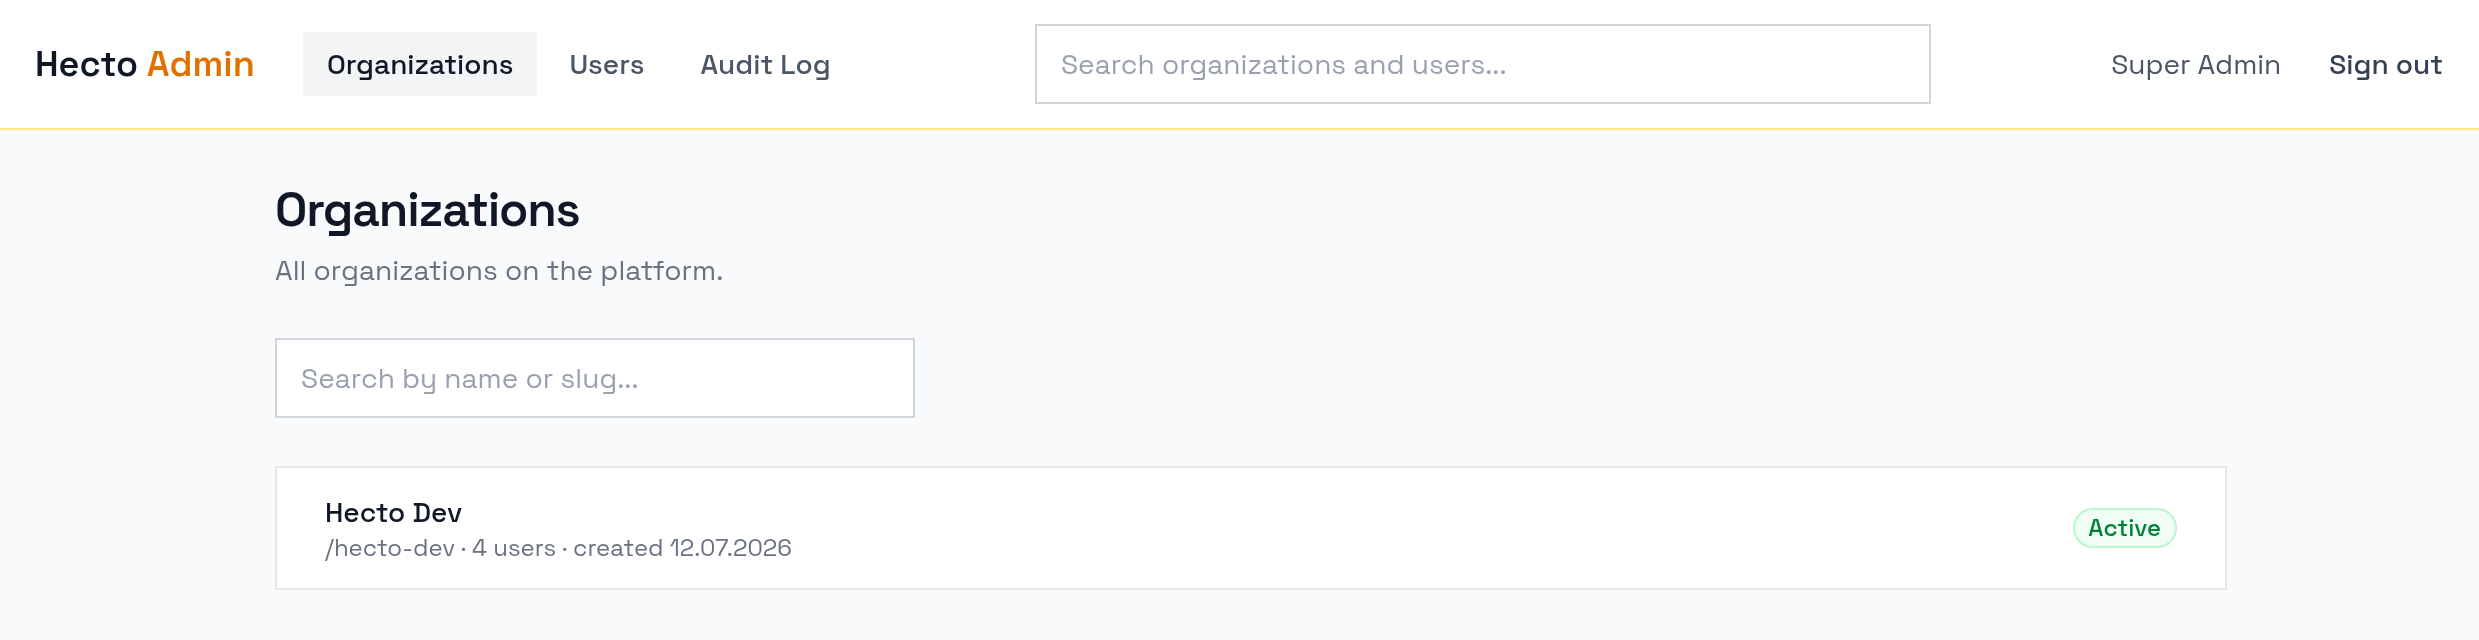
\includegraphics[width=\textwidth]{slike/admin-organizacije.png}
\caption{Pregled organizacij v administratorski aplikaciji.}
\label{fig:admin-organizacije}
\end{figure}
\FloatBarrier
